\section{Legendre Polynomials}
\label{sec:legendre}

Legendre polynomails are solutions to {\em Legendre's differential
  equation},
\begin{equation}
  \label{eq:legendrede}
  \frac{\dif{}}{\dif{x}} \left[ (1-x)^2 \frac{\dif{}}{\dif{x}} P_n(x) \right] + n(n+1) P_n(x) = 0
\end{equation}
These are encountered frequently when solving Laplace's equation in
spherical coordinates. This differential equation can be solved using
a power series method. The equation has regualr singular points at
$x=\pm 1$, so solutions only converge in the region $|x|<1$. When $n$
is an integer, the solution $P_n(x)$ that is regular at $x=1$ is also
regular at $x=-1$, and the solution terminates. These solutions,
$P_n$, are called the {\em Legendre Polynomials}, with each being an
$n^{\rm th}$-degree polynomial, expressed by Rodrigues' Formula:
\begin{equation}
  \label{eq:rodrigues}
  P_n(x) = \frac{1}{2^n\ n!} \frac{\difp{n}{}}{\difp{n}{x}} \left[ (x^1-1)^n \right]
\end{equation}

\subsection{Legendre Polynomials from the Generating Function}
\label{sec:generatinglegendre}

\begin{definition}[Formal Power Series]
  A formal power series is a generalisation of the concept of a
  polynomial, where the number of terms is allowed to be infinite.
\end{definition}
A formal power series can be considered in the same way as a normal
power series, but we ignore considerations of the convergence by
assuming that a variable, $X$, denotes any numerical value. For
example, the series
\[ A = 1 - 3X+ 5X^2 - 7X^3 + 9X^4 - 11X^5 + \cdots \] As a power
series, one property of this series is that it has a radius of
convergence equal to 1. As a formal power series the only relevent
information is that the sequence of coefficients, $[1, -3, 5, -7, 9,
-11, \dots]$. Thus a formal power series merely records the sequence
of coefficients.

\begin{definition}[Generating Function]
  A generating function is a formal power series in one indeterminate,
  the coefficients of which encode information about a sequence of
  numbers, $a_n$, which is indexed by natural numbers.
\end{definition}

The Legendre Polynomials can be described by a generating function,
$g(t,x)$,
\begin{equation}
  \label{eq:legendregen}
  g(t,x) = \frac{1}{\sqrt{1- 2xt +t^2}} = \sum^{\infty}_{n=0} P_n(x) t^n
\end{equation}
It is then possible to find expressions for the Legendre polynomials
by expanding the square root in powers of $t$, and equating
coefficients:
\begin{align*}
  (1-2xt+t^2)^{-\frac{1}{2}} &= 1 + \frac{1}{2}(2xt -t^2)+\frac{3}{8}(2xt-t^2)^2\\&\quad +\frac{5}{16}(2xt-t^2)^3 + \frac{35}{128}(2xt-t^2)^4 \\ &\quad + {\cal O}(t^5)\\
  \text{and,}\quad \sum^{\infty}_{n=0} P_n(x) t^n &= t^0 + xt^1 +
  \frac{1}{2}(3x^2-1)t^2 \\&\quad \frac{1}{2}(5 x^3-3)t^3 +
  \frac{1}{8}(35x^4-30x^2+3)t^4 \\&\quad + {\cal O}(t^5)
\end{align*}
so, by equating the appropriate powers of $t$,
\begin{align*}
  P_0(x) &= 1 \\
  P_1(x) &= x \\
  P_2(x) &= \frac{1}{2}(3 x^2 - 1) \\
  P_3(x) &= \frac{1}{2}(5 x^3 - 3x) \\
  P_4(x) &= \frac{1}{8}(35 x^4 - 30x^2 + 3)
\end{align*}
\begin{figure}
  \centering \begin{centering}
\begin{tikzpicture}[scale=1.0]
%\draw[help lines] (0,0) grid (8,3);
\begin{axis}[width=\linewidth, height=2in, xmin=-1, xmax=1, samples=50]%[hide axis, axis on top]

    \addplot gnuplot[raw gnuplot, id=leg1, mark=none, domain=-1:1, muted-blue, ultra thick]{
    	     set xrange [-1:1];
    	     leg(n,x) = (n==0) ? 1 : (n==1) ? x : ((2*n+1)*x*leg(n-1, x) - n*leg(n-2, x))/(n+1);
	     plot leg(0,x);
    };
    \addplot gnuplot[raw gnuplot, id=leg2, mark=none, domain=-1:1, muted-green, ultra thick]{
    	     set xrange [-1:1];
    	     leg(n,x) = (n==0) ? 1 : (n==1) ? x : ((2*n+1)*x*leg(n-1, x) - n*leg(n-2, x))/(n+1);
	     plot leg(1,x);
    };
    \addplot gnuplot[raw gnuplot,mark=none, id=leg3, domain=-1:1, muted-orange, ultra thick]{
    	     set xrange [-1:1];
    	     leg(n,x) = (n==0) ? 1 : (n==1) ? x : ((2*n+1)*x*leg(n-1, x) - n*leg(n-2, x))/(n+1);
	     plot leg(2,x);
    };
    \addplot gnuplot[raw gnuplot, mark=none, id=leg4, domain=-1:1, accent-purple, ultra thick]{
    	     set xrange [-1:1];
    	     leg(n,x) = (n==0) ? 1 : (n==1) ? x : ((2*n+1)*x*leg(n-1, x) - n*leg(n-2, x))/(n+1);
	     plot leg(3,x);
    };
    \addplot gnuplot[raw gnuplot, mark=none, id=leg5, domain=-1:1, accent-red, ultra thick]{
    	     set xrange [-1:1];
    	     leg(n,x) = (n==0) ? 1 : (n==1) ? x : ((2*n+1)*x*leg(n-1, x) - n*leg(n-2, x))/(n+1);
	     plot leg(4,x);
    };
\end{axis}
\end{tikzpicture}
\end{centering}
  \caption{The first 5 Legendre Polynomials}
  \label{fig:legendrepoly}
\end{figure}

\subsection{Parity of Legendre Polynomials}
\label{sec:parity}

At $x = \pm 1$ the situation is especially simple;
\begin{align*}
  g(t, \pm 1) &= \frac{1}{\sqrt{1 \mp 2t + t^2}} = \frac{1}{\sqrt{(1 \mp t)^2}} \\
  &= 1 \pm t +t^2 \pm t^3 + \cdots \\
  &= \sum_{n=0}^{\infty} (\pm 1)^n t^n
\end{align*}
but also
\begin{align*}
  g(t, \pm 1) &= \sum^{\infty}_{n=0} P_n(\pm 1) t^n \\
  P_n(1) &=1 \\
  P_n(-1)&=(-1)^n =
  \begin{cases}
    +1 & \text{ for } n \text{ even.} \\
    -1 & \text{ for } n \text{ odd.}
  \end{cases}
\end{align*}
And
\begin{align*}
  g(-t,-x) &= \frac{1}{\sqrt{1-2(-x)(-t)+(-t)^2}} = \frac{1}{\sqrt{1-2xt+t^2}} \\
  &= g(t,x)
\end{align*}
Then, equating powers of $t$,
\[ P_n(-x) = (-1)^nP_n(x) \]

\subsection{Legendre Polynomials and Multipole Expansion}
\label{sec:multipolelegendre}

Consider a point charge, $q$, on the $z$-axis, a distance $a$ from the
origin. The potential at an arbitrary point $\vec{r}$ will be
\begin{align*}
  \phi(\vec{r}) &= \frac{1}{4 \pi \epsilon_0} \frac{q}{d} = \frac{1}{4 \pi \epsilon_0} \frac{q}{|\vec{r} - a \hat{e}_z|} \\
                &= \frac{1}{4 \pi \epsilon_0} \frac{q}{\sqrt{(\vec{r}-a \hat{e}_z)\cdot(\vec{r}-a \hat{e}_z)}}\\
                &= \frac{1}{4 \pi \epsilon_0} \frac{q}{\sqrt{r^2-2ra \cos \theta + a^2}}\\
                &= \frac{q}{4 \pi \epsilon_0 r} \qty[  1 - 2 \frac{a}{r} \cos \theta + \qty(\frac{a}{r})^2 ]^{-\frac{1}{2}}\\
                &= \frac{q}{4 \pi \epsilon_0 r} \sum_{n=0}^{\infty} P_n(\cos \theta)
  \qty( \frac{a}{r})^n
  \end{align*}
  Adding an extra point charge, $-q$ a distance $a$ on the opposite
  size of the origin gives us
  \begin{align*}
   \phi(\vec{r})  &= \frac{1}{4 \pi \epsilon_0} \frac{q}{d_1} - \frac{1}{4 \pi \epsilon_0} \frac{q}{d_2} \\
                  &= \frac{1}{4 \pi \epsilon_0} \frac{q}{|\vec{r}-a \vec{e}_z|} - \frac{1}{4 \pi \epsilon_0} \frac{q}{|\vec{r}+a \vec{e}_z|} 
\\                &= \frac{q}{4 \pi \epsilon_0 r} \bigg[ \left(1-2 \frac{a}{r} \cos \theta +\left(\frac{a}{r}\right)^2 \right)^{-\frac{1}{2}} 
\\                &  \qquad \qquad -  \left(1-2 \frac{a}{r} \cos \theta +\left(\frac{a}{r}\right)^2 \right)^{-\frac{1}{2}} \bigg] 
\\                &= \frac{q}{4 \pi \epsilon_0 r} \sum_{n=0}^{\infty} \qty( P_n(\cos\theta) \qty( \frac{a}{r} )^n - P_n(\cos \theta) \qty( \frac{-a}{r})^n )
\\                &= \frac{2q}{4 \pi \epsilon_0 r} \qty( P_1 (\cos \theta) \frac{a}{r} + P_3 (\cos \theta) \qty(\frac{a}{r})^3 + \cdots )
    \end{align*}
    so, only odd powers survive, and, for large enough $r$,
    \[ \phi(\vec{r}) \approx \frac{2qa}{4 \pi \epsilon_0 r^2}
    P_1(\cos\theta) \] This is the potential from an electric dipole,
    and $2qa$ is the dipole moment.  The leading term in an expansion
    describes the distribution:
    \begin{align*}
      \frac{1}{r} P_0 (\cos \theta) \left(\frac{a}{r}\right)^0 &= \frac{1}{r} & \text{(Monopole)} \\
      \frac{1}{r} P_1 (\cos \theta) \left(\frac{a}{r}\right)^1 &= \frac{a}{r^2} \cos \theta & \text{(Dipole)} \\
      \frac{1}{r} P_2 (\cos \theta) \left(\frac{a}{r}\right)^2 &= \frac{a^2}{2r^3} (3\cos^2 \theta - 1) & \text{(Quadrupole)} \\
      \frac{1}{r} P_3 (\cos \theta) \left(\frac{a}{r}\right)^3 &= \frac{a^3}{2r^4} (5\cos^3 \theta - 3 \cos \theta) & \text{(Octupole)} \\
    \end{align*}

    \subsection{Recurrence Relations for Legendre Polynomials}
    \label{sec:recurrencelegendre}

    We can derive recurrence relations for the Legendre polynomials
    starting by taking the derivative of the generating function,
    equation (\ref{eq:legendregen}).
    \begin{align*}
      \frac{\partial g(t,x)}{\partial t} &= \frac{x-t}{(1-2xt+t^2)^{\frac{3}{2}}} = \sum_{n=0}^{\infty} P_n(x)nt^{n-1} \\
      &= \frac{x-t}{(1-2xt+t^2)}\frac{1}{\sqrt{1-2xt+t^2}} \\
      &= \frac{x-t}{1-2xt+t^2} \sum_{n=0}^{\infty}P_n(x) t^n \\
    \end{align*}
    Thus
    \begin{align*}
      (1-2xt+t^2) \sum_{n=0}^{\infty} P_n(x) nt^{n-1} &= (x-t)
      \sum_{n=0}^{\infty} P_n(x) t^n
    \end{align*}
    expanding,
    \begin{align*}
      \sum_{n=0}^{\infty} P_n(x) nt^{n-1} &- sx \sum_{n=0}^{\infty} P_n(x) nt^n + \sum_{n=0}^{\infty} P_n(x) nt^{n+1} \\
      &= x \sum_{n=0}^{\infty} P_n(x)t^n - \sum_{n=0}^{\infty} P_n(x)
      t^{n+1}
    \end{align*}
    Then, relabelling,
    \begin{align*}
      \sum_{n=-1}^{\infty} P_{n+1}(x)(n+1) &- 2x \sum_{n=0}^{\infty} P_n(x) nt^n + \sum_{n=1}^{\infty} P_{n-1}(x)(n-1) \\
      &= x \sum_{n=0}^{\infty} P_n(x) t^n - \sum_{n=1}^{\infty}
      P_{n-1}(x) t^n
    \end{align*}
    Equating powers of $t^n$ for $n \ge 1$,
    \[ P_{n+1}(x)(n+1) - 2x P_n(x)n + P_{n-1}(x)(n-1) = xP_n(x) -
    P_{n-1}(x) \] Thus
    \[ (2n+1) x P_n(x) = (n+1) P_{n+1}(x) + nP_{n-1}(x) \qquad (n \ge
    1) \] This recurrence relation allows the calculation of Lengendre
    polynomials using a recursive function.  Taking the derivative
    with respect to $x$ instead,

\begin{align*}
  \frac{\partial g(t,x)}{\partial x} &= \frac{t}{(1-2xt +t^2)^{\frac{3}{2}}} \\
  &= \sum_{n=0}^{\infty} P^{\prime}_n(x)t^n \\
  &= \frac{t}{1-2xt+t^2} \frac{1}{\sqrt{1-2xt+t^2}} \\
  &= \frac{t}{1-2xt+t^2} \sum_{n=0}^{\infty} P_n(x) t^n \\
  (1-2xt+t^2) \sum_{n=0}^{\infty} P^{\prime}_n(x)t^n &= t
  \sum_{n=0}^{\infty} P_n(x) t^n
\end{align*}
\[ P^{\prime}_{n+1}(x) + P^{\prime}_{n-1}(x) = 2x P_n^{\prime}(x) +
P_n(x) \]

\subsection{Orthogonality and Completeness of the Legendre
  Polynomials}
\label{sec:orthogonallegendre}

It is possible to show that the Legendre Polynomials are orthogonal by
considering the Legendre equation, equation (\ref{eq:legendrede}).
\begin{align*}
  P_m(x) & \textcolor{accent-red}{\frac{\dif{}}{\dif{x}} \left[ (1-x^2) \frac{\dif{}}{\dif{x}}P_n(x)\right]} - P_n(x) \textcolor{accent-blue}{\frac{\dif{}}{\dif{x}}\left[ (1-x^2) \frac{\dif{}}{\dif{x}}P_m(x) \right]} \\
  &= - P_m(x) \textcolor{accent-red}{n(n+1)P_n(x)}+P_n(x)
  \textcolor{accent-blue}{m(m+1)P_m(x)}
\end{align*}
Now, integrating $x$ over the range $[-1, 1]$,
\begin{align*}
  \int_{-1}^1& \textcolor{accent-blue}{P_m(x)} \frac{\dif{}}{\dif{x}}
  \left[ \textcolor{accent-red}{(1-x^2) \frac{\dif{}}{\dif{x}} P_n(x)}
  \right] \dif{x} \\= & \underbrace{\left[
      \textcolor{accent-blue}{P_m(x)} \textcolor{accent-red}{(1-x)^2
        \frac{\dif{}}{\dif{x}}P_n(x)} \right]^1_{-1}}_{= 0} \\ &-
  \underbrace{\int_{-1}^1 \left[ \frac{\dif{}}{\dif{x}}
      \textcolor{accent-blue}{P_m(x)}\textcolor{accent-red}{(1-x^2)
        \frac{\dif{}}{\dif{x}} P_n(x)} \right]
    \dif{x}}_{\text{symmetric in n,m}} \\0 & = [m(m+1) - n(n+1)]
  \int_{-1}^1 P_n(x) P_m(x) \dif{x}
\end{align*}
Then, for $n \neq m$,
\[ \int_{-1}^1 P_n(x) P_m(x) \dif{x} = 0 \] So Legendre polynomials
are orthogonal over the region $x \in [-1, 1]$ When $n=m$, we return
to the generating function,
\[ \sum_{n=0}^{\infty} P_n(x)t^n \sum_{m=0}^{\infty} P_m(x)t^m =
\frac{1}{1-2xt+t^2} \] Integrating over $x$,
\begin{align*}
  \int_{-1}^1 \frac{1}{1-2xt+t^2} \dif{x} &= \left[ - \frac{1}{2t}
    \log (1-2xt+t^2) \right]^1_{-1} \\ &= \frac{1}{t} \log \left(
    \frac{1+t}{1-t} \right) \\ &= 2 \sum_{n=1}^{\infty}
  \frac{t^{2n}}{2n+1}
\end{align*}

\begin{align*}
  \int_{-1}^1 \sum_{n=0}^{\infty} P_n(x)t^n \sum_{m=0}^{\infty} P_m(x)
  t^m \dif{x} &= \sum_{n=0}^{\infty} \int_{-1}^1 [P_n(x)]^2 t^{2n}
  \dif{x}
\end{align*}

and equating powers of $t$,
\begin{align*}
  \int_{-1}^1 [P_n(x)]^2 \dif{x} = \frac{2}{2n + 1}
\end{align*}
And putting these relations together we get an orthogonality and
normalisation condition
\begin{equation}
  \label{eq:orthonormlegend}
  \int_{-1}^1 P_n(x) P_m(x) \dif{x} = \frac{2}{2n+1} \delta_{nm}
\end{equation}
Legendre polynomials are also complete---any continuous function can
be expressed as an infinite sum of Legendre polynomials in $x \in
[-1,1]$. Taking a function $f(x)$, then
\begin{equation}
  \label{eq:legendreseries}
  f(x) = \sum_{n=0}^{\infty} c_n P_n(x)
\end{equation}
Then,
\begin{align*}
  \int_{-1}^1 f(x) P_m(x) \dif{x} &= \sum_{n=0}^{\infty} c_n
  \int_{-1}^1 P_n(x) P_m(x) \dif{x} \\ &= \sum_{n=0}^{\infty} c_n
  \frac{2}{2m+1} \delta_{nm} \\ &= c_m \frac{2}{2m+1}
\end{align*}
So,
\begin{equation}
  \label{eq:legendreseriesoffunc}
  f(x) = \sum_{n=0}^{\infty} \left( n + \frac{1}{2} \right) \left( \int_{-1}^1 f(y) P_n(y) \dif{y} \right) P_n(x)
\end{equation}
\begin{example}
  {\em Expanding the step function as a series of Legendre polynomials.}\\
  \begin{centering}
\begin{tikzpicture}[scale=1.0]
%\draw[help lines] (0,0) grid (8,3);
\begin{axis}[width=\linewidth, height=2in, xmin=-1, xmax=1, samples=50]%[hide axis, axis on top]
    \addplot gnuplot[raw gnuplot, id=leg1, mark=none, domain=-1:1, muted-blue, ultra thick]{
    	     set xrange [-1:1];
    	     step(x) = (x>0) ? 1 : 0;
	     plot step(x);
    };
\end{axis}
\end{tikzpicture}
\end{centering}\\
  We have the definition of a Legendre series from equation (\ref{eq:legendreseriesoffunc}) as
  \[ f(x) = \sum_l c_l P_l(x) \]
  then
  \begin{align*} 
\int_{-1}^1 f(x) P_m(x) \dd{x} &= \sum_{l=0}^{\infty} c_l \int_{-1}^1 P_l(x) P_m(x) \dd{x} \\&= c_m \frac{2}{2m+1}
\end{align*}
and so
  \[ c_l = \frac{2l+1}{2} \int_{-1}^1 f(x) P_l(x) \dd{x} \]
  now
  \begin{align*}
    c_0 &= \frac{1}{2} \int_0^1 P_0(x) \dd{x} = \frac{1}{2} \\
    c_1 &= \frac{3}{2} \int_0^1 P_1(x) \dd{x} = \frac{3}{4} \\
  \end{align*}
  and so
  \begin{equation*}
    f(x) = \frac{1}{2} P_0(x) + \frac{3}{4} P_1(x) - \frac{7}{16} P_3(x) + \frac{11}{32} P_5(x) + \cdots
  \end{equation*}
  \begin{centering}
\begin{tikzpicture}[scale=1.0]
%\draw[help lines] (0,0) grid (8,3);
\begin{axis}[width=\linewidth, height=2in, xmin=-1, xmax=1, samples=50]%[hide axis, axis on top]
    \addplot gnuplot[raw gnuplot, id=leg1, mark=none, domain=-1:1, muted-orange, ultra thick]{
    	     set xrange [-1:1];
    	     leg(n,x) = (n==0) ? 1 : (n==1) ? x : ((2*n+1)*x*leg(n-1, x) - n*leg(n-2, x))/(n+1);
	     plot ( 0.5*leg(0,x)+0.75*leg(1,x)-(0.4375)*leg(3,x)+(0.34375)*leg(5,x) );
    };
\end{axis}
\end{tikzpicture}
\end{centering}
\end{example}

\section{Associated Legendre Polynomials}
\label{sec:assocpolynomials}

Associated Legendre polynomials are obtained by differentiating a
standard Legendre polynomial $m$ times, with respect to $x$.
\begin{equation}
  \label{eq:definitionassocleg}
  P_n^m(x) = (1-x^2)^{\frac{m}{2}} \frac{\dif{}^m}{\dif{x}^m} P_n(x)
\end{equation}
these are solutions of the associate Legendre equation,
\begin{equation}
  \label{eq:assoclegendrede}
  \frac{\dif{}}{\dif{x}} \left[ (1-x^2) \frac{\dif{P_n^m(x)}}{\dif{x}} \right] + n(n+1)P_n^m(x) - \frac{m^2}{1-x^2} P_n^m(x) = 0
\end{equation}

\begin{figure}
  \centering
  \begin{tikzpicture}
    \begin{axis}[width=\linewidth, height=2in, xmin=-1, xmax=1]
      \addplot shell [prefix=pgfshell_, id=leg, mark=none, muted-blue, ultra thick]{\python{1}{0}};
      \addplot shell [prefix=pgfshell_, id=leg, mark=none, muted-green, ultra thick]{\python{1}{1}};
      \addplot shell [prefix=pgfshell_, id=leg, mark=none, muted-orange, ultra thick]{\python{1}{2}};
      \addplot shell [prefix=pgfshell_, id=leg, mark=none, accent-purple, ultra thick]{\python{1}{3}};
      \addplot shell [prefix=pgfshell_, id=leg, mark=none, accent-red, ultra thick]{\python{1}{4}};
    \end{axis}
  \end{tikzpicture}
\begin{tikzpicture}
    \begin{axis}[width=\linewidth, height=2in, xmin=-1, xmax=1]
      \addplot shell [prefix=pgfshell_, id=leg, mark=none, muted-blue, ultra thick]{\python{1}{1}};
      \addplot shell [prefix=pgfshell_, id=leg, mark=none, muted-green, ultra thick]{\python{1}{2}};
      \addplot shell [prefix=pgfshell_, id=leg, mark=none, muted-orange, ultra thick]{\python{1}{3}};
      \addplot shell [prefix=pgfshell_, id=leg, mark=none, accent-purple, ultra thick]{\python{1}{4}};
      \addplot shell [prefix=pgfshell_, id=leg, mark=none, accent-red, ultra thick]{\python{1}{5}};
    \end{axis}
  \end{tikzpicture}
\begin{tikzpicture}
    \begin{axis}[width=\linewidth, height=2in, xmin=-1, xmax=1]
      \addplot shell [prefix=pgfshell_, id=leg, mark=none, muted-blue, ultra thick]{\python{2}{2}};
      \addplot shell [prefix=pgfshell_, id=leg, mark=none, muted-green, ultra thick]{\python{2}{3}};
      \addplot shell [prefix=pgfshell_, id=leg, mark=none, muted-orange, ultra thick]{\python{2}{4}};
      \addplot shell [prefix=pgfshell_, id=leg, mark=none, accent-purple, ultra thick]{\python{2}{5}};
      \addplot shell [prefix=pgfshell_, id=leg, mark=none, accent-red, ultra thick]{\python{2}{6}};
    \end{axis}
  \end{tikzpicture}
\begin{tikzpicture}
    \begin{axis}[width=\linewidth, height=2in, xmin=-1, xmax=1]
      \addplot shell [prefix=pgfshell_, id=leg, mark=none, muted-blue, ultra thick]{\python{3}{3}};
      \addplot shell [prefix=pgfshell_, id=leg, mark=none, muted-green, ultra thick]{\python{3}{4}};
      \addplot shell [prefix=pgfshell_, id=leg, mark=none, muted-orange, ultra thick]{\python{3}{5}};
      \addplot shell [prefix=pgfshell_, id=leg, mark=none, accent-purple, ultra thick]{\python{3}{6}};
      \addplot shell [prefix=pgfshell_, id=leg, mark=none, accent-red, ultra thick]{\python{3}{7}};
    \end{axis}
  \end{tikzpicture}
\begin{tikzpicture}
    \begin{axis}[width=\linewidth, height=2in, xmin=-1, xmax=1]
      \addplot shell [prefix=pgfshell_, id=leg, mark=none, muted-blue, ultra thick]{\python{4}{4}};
      \addplot shell [prefix=pgfshell_, id=leg, mark=none, muted-green, ultra thick]{\python{4}{5}};
      \addplot shell [prefix=pgfshell_, id=leg, mark=none, muted-orange, ultra thick]{\python{4}{6}};
      \addplot shell [prefix=pgfshell_, id=leg, mark=none, accent-purple, ultra thick]{\python{4}{7}};
      \addplot shell [prefix=pgfshell_, id=leg, mark=none, accent-red, ultra thick]{\python{4}{8}};
    \end{axis}
  \end{tikzpicture}
  \caption{The associated Legendre Polynomials}
  \label{fig:assoclegendre}
\end{figure}

Then,
\[ P_0(x) = 1 \therefore P_0^0(x) = 1 \]
\[ P_1(x) = x \therefore P_1^0(x) = x \]
\[ P_1^1(x) = (1-x^2)^{\frac{1}{2}} \]

There are different conventions for negative values of $m$, but since
the only dependence on $m$ is an $m^2$ term, we can take them to be
equal.  If $x = \cos (\theta)$,
\[ P_1^0(x) = \cos(\theta) \]
\[ P_1^{\pm 1} = \sin(\theta) \]
The associated Legendre polynomials are also orthogonal,
\begin{equation}
  \label{eq:orthogonalityassoclag}
  \int_{-1}^1 P_l^m(x) P_n^m(x) \dd{x} = \frac{(l+m)!}{(l-m)!} \frac{2}{2l+1} \delta_{ln}
\end{equation}


\subsection{Spherical Harmonics}
\label{sec:spharmonics}
Spherical harmonics are a class of function related to the associated Legendre polynomials by the expression
\begin{equation}
  \label{eq:spharmonicdef}
  Y_{lm}(\theta, \phi) = \qty[ \frac{2l+1}{4 \pi} \frac{(l-|m|)!}{(l+|m|)!}]^{\frac{1}{2}} P_l^m (\cos(\theta)) e^{im\phi}
\end{equation}

\begin{figure*}
  \centering
  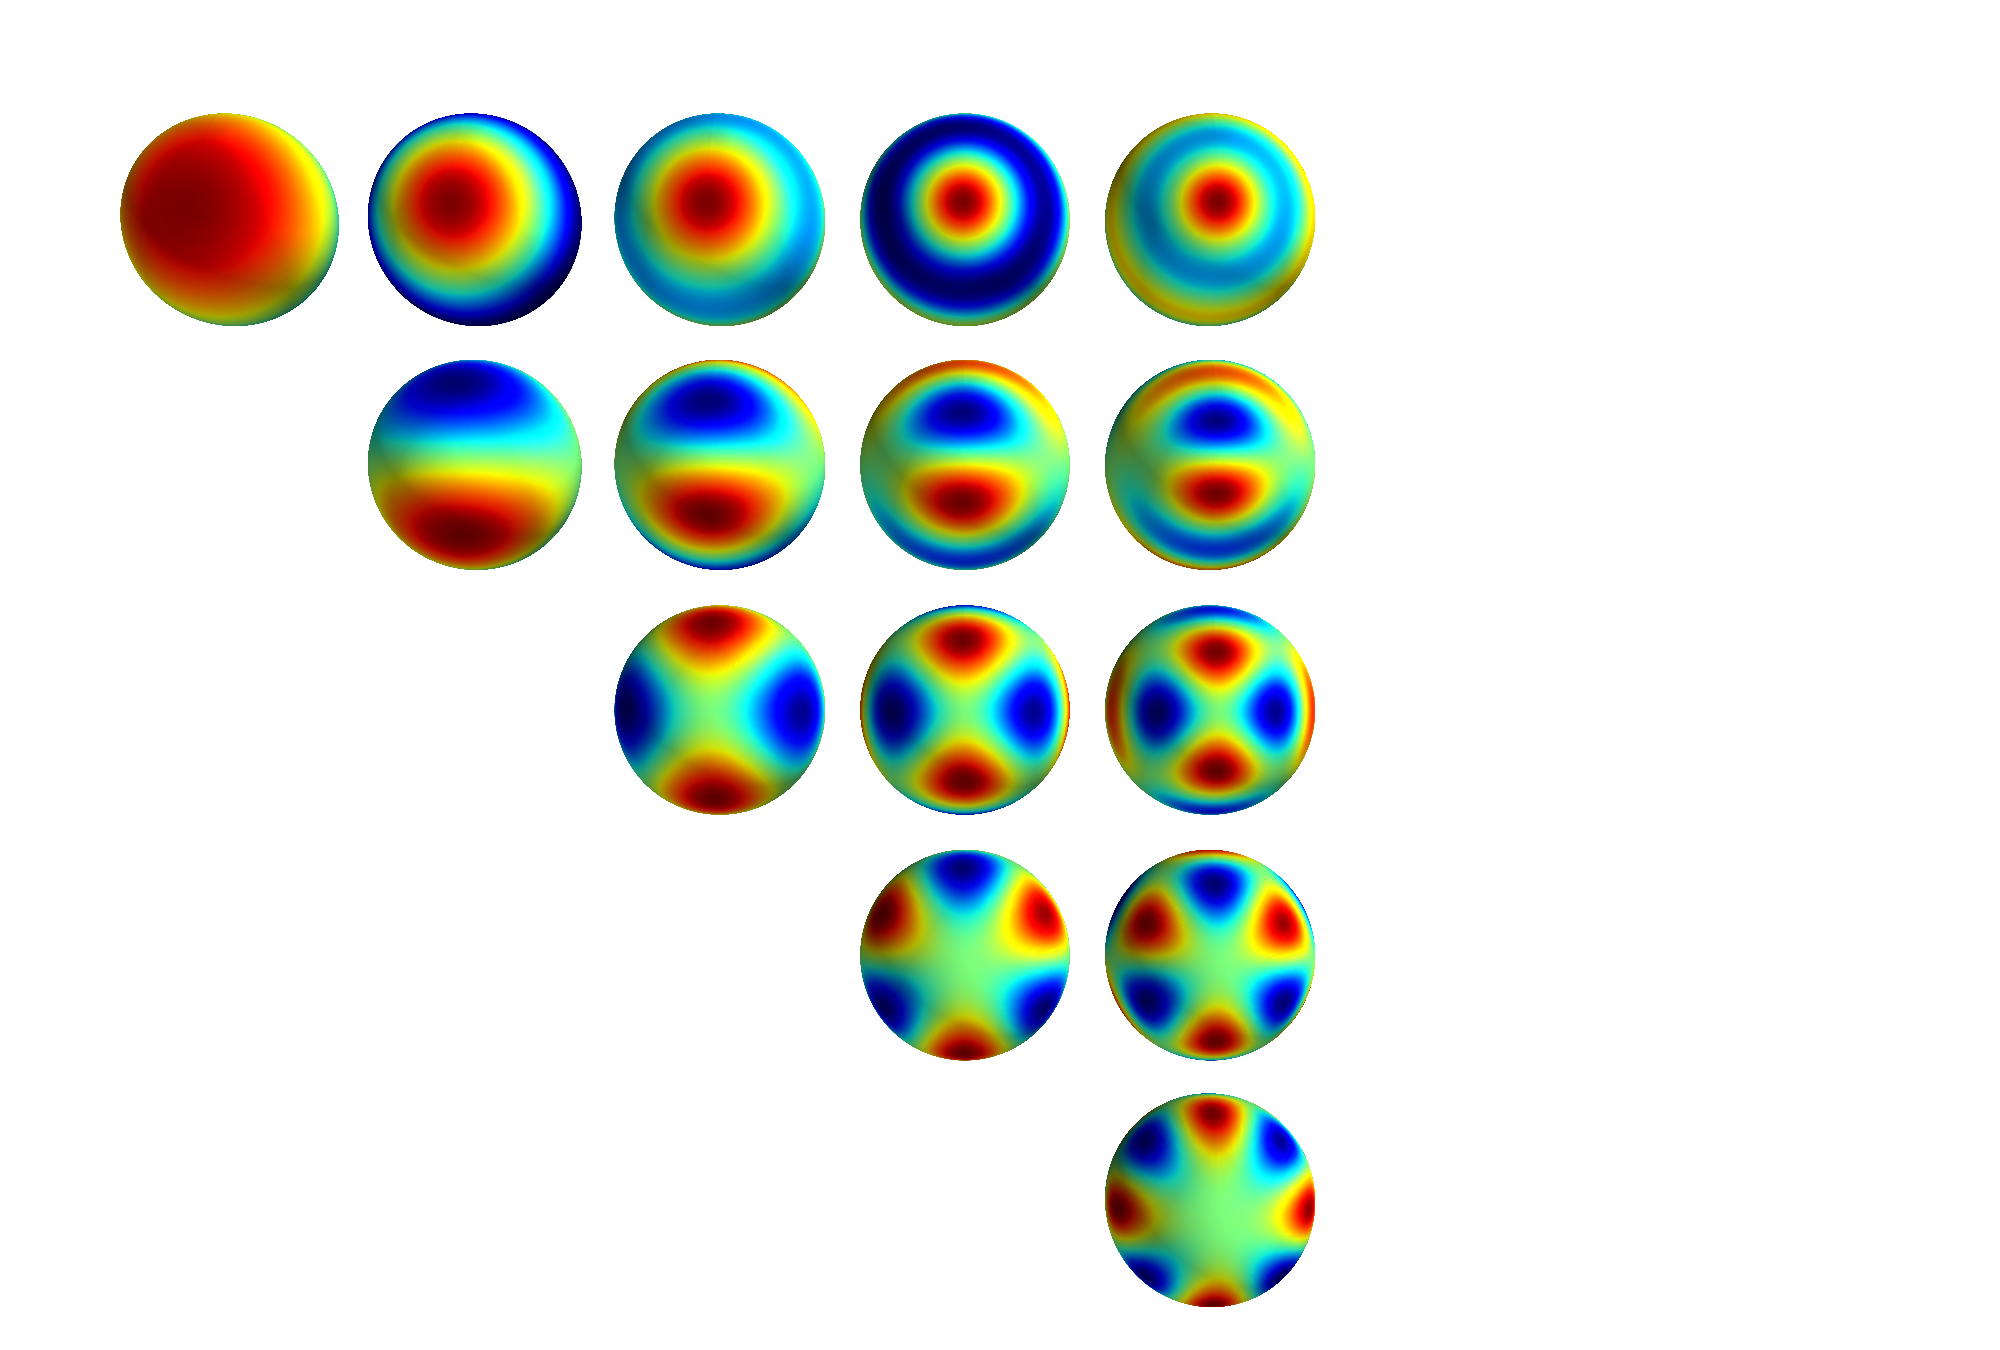
\includegraphics[width=\textwidth]{figures/spharmonics.png}
  \caption{Spherical Harmonics}
  \label{fig:spharmonics}
\end{figure*}

\begin{figure*}
  \centering
  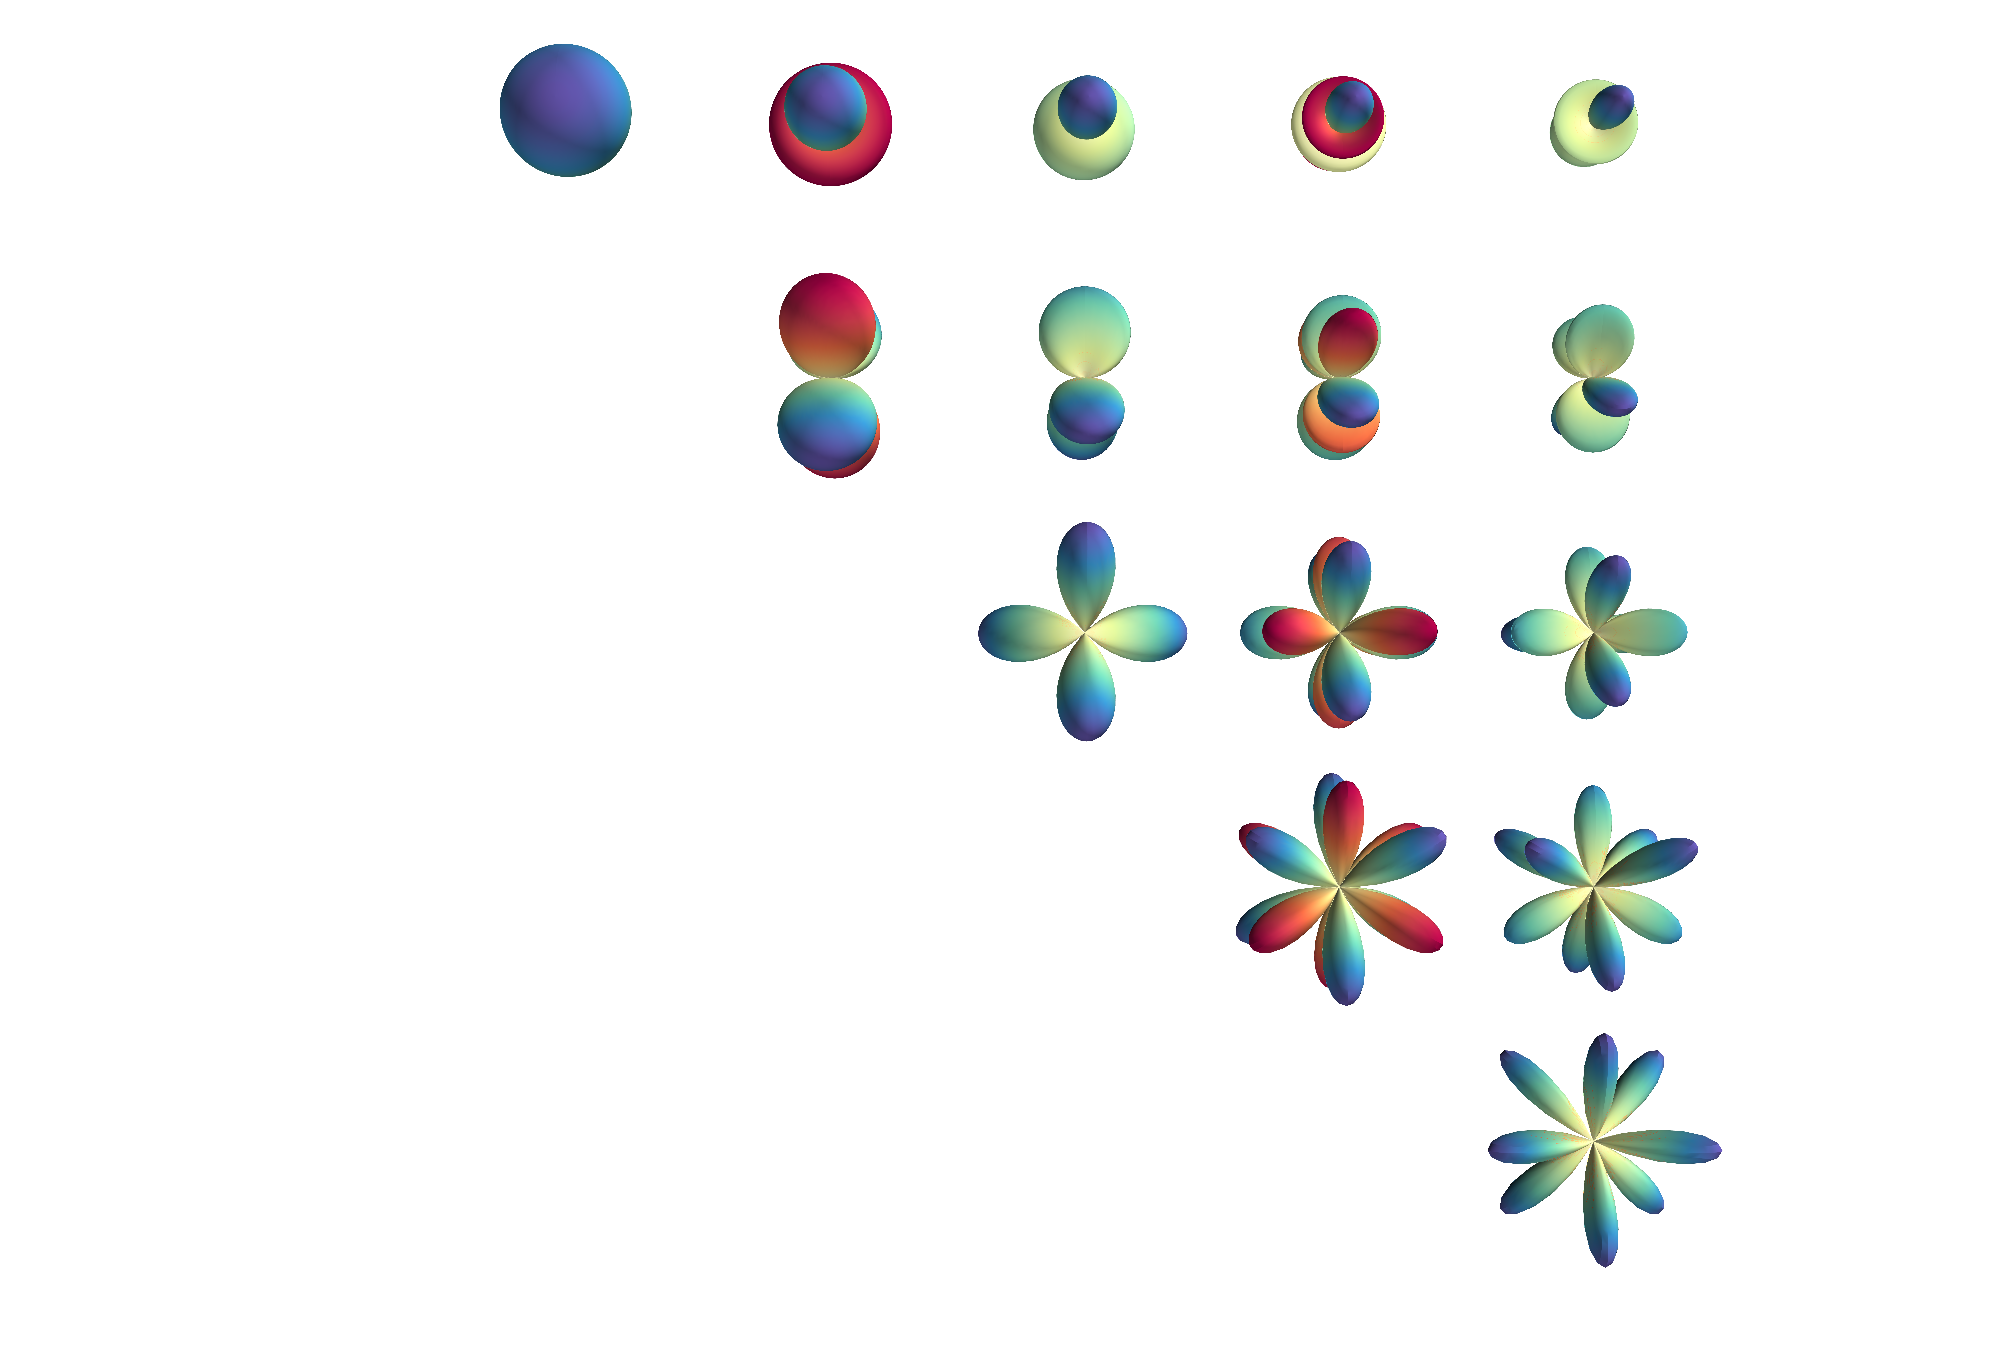
\includegraphics[width=\textwidth]{figures/spharmonics2.png}
  \caption{An alternative representation of Spherical Harmonics}
  \label{fig:spharmonics}
\end{figure*}

Spherical harmonics with a negative $m$ value can be related to those
with a positive $m$ value via
\begin{equation}
  \label{eq:negativespharm}
  Y_{l, -m} (\theta, \phi) = (-1)^m Y^{*}_{lm} (\theta, \phi)
\end{equation}
and they are orthogonal,
\begin{equation}
  \label{eq:spahrmorthog}
  \int \dd{\Omega} Y^{*}_{lm} (\theta, \phi) Y_{l^{\prime}m^{\prime}}(\theta, \phi) = \delta_{l l^{\prime}} \delta_{m, m^{\prime}}
\end{equation}
The first few spherical harmonics are
\[ Y_{00} = \sqrt{\frac{1}{4 \pi}} \]
\[ Y_{10}= \sqrt{\frac{3}{4 \pi}} \cos(\theta) \]
\[ Y_{1, \pm 1} = \mp \sqrt{\frac{3}{8 \pi}} \sin(\theta) e^{\pm i \phi} \]

\subsection{Spherical Harmonics and the Schrodinger Equation}
\label{sec:spherharmschrod}

In spherical coordinates the time-independent Schrodinger equation is
\begin{equation}
  \label{eq:tisespherical}
  \begin{split}
  - \frac{\hbar^2}{2m} \frac{1}{r^2 \sin^2 \theta} \bigg( \pdv{r} \qty[ r^2 \sin(\theta) \pdv{\psi}{r}] 
+ \pdv{\theta} \qty[ \sin \theta  \pdv{\psi}{\theta}] \\ + \pdv{\phi} \qty[ \frac{1}{\sin \theta} \pdv{\psi}{\phi}] \bigg) 
+ (V-E)\psi = 0
\end{split}
\end{equation}
Now, splitting this into the radial part and an angular part,
\begin{equation}
  \label{eq:sepschrod}
  \psi(r, \theta, \phi) = R(r) Y(\theta, \phi)
\end{equation}
Then, substituting this in, and setting both sides of the equation
equal to $l(l+1)$ we get two independent solutions
\begin{align}
  \dv{r} \qty[r^2 \dv[2]{R}{r}] - \frac{2m}{\hbar^2} \qty(V(r)-E) r^2
  R - l(l+1) R &= 0 \\\frac{1}{\sin \theta} \pdv{\theta} \qty[ \sin
  \theta \pdv{Y}{\theta}] + \frac{1}{\sin^2(\theta)}
  \pdv[2]{Y}{\phi} +l(l+1)Y &= 0
\end{align}
The angular part is solved by spherical harmonics,
\begin{equation}
  \label{eq:sphericalharmonics}
  Y_l^m(\theta, \phi) = N e^{im\phi} P_l^m (\cos \theta)
\end{equation}

\section{Bessel Functions}
\label{sec:bessel}

Bessel functions are the solutions to Bessel's differential equation,
\begin{equation}
  \label{eq:besselde}
  x^2 \dv[2]{y}{x} + x \dv{y}{x} + (x^2 - \alpha^2)y = 0
\end{equation}
with $p$ a constant. 

\subsection{Bessel functions from the Generating Function}
\label{sec:besselgen}

The Bessel functions can be described by a generating function,
\begin{equation}
  \label{eq:besselgen}
  g(x,t) = \exp(\frac{x}{2t}(t^2-1)) = \sum_{\nu=-\infty}^{\infty} J_{\nu}(x) t^{\nu}
\end{equation}

So, for Bessel functions of integer order we can expand this to form a series expansion,
\begin{equation}
  \label{eq:besselseriesexp}
  J_n(x) = \sum^{\infty}_{s=0} \frac{(-1)^s}{s! (n+s)!} \qty( \frac{x}{2} )^{n+2s} \approx \frac{x^n}{2^n n!}
\end{equation}
for small $x$.

Bessel functions with a negative index can be found from the relation
\begin{equation}
  \label{eq:negativebessel}
  J_{-\nu}(x) = (-1)^{\nu} J_{\nu}(x)
\end{equation}

\begin{figure}
  \centering
  \begin{tikzpicture}
    \begin{axis} [
    width=\linewidth, height=2in,
    xmin=0, xmax=20,
%   xtick={7700,7725,...,7800},
%   ymin=0.009, ymax=0.05,
    ]
    \addplot gnuplot[raw gnuplot, id=bess, mark=none, muted-blue, ultra thick]{
      set xrange[0:20];
      plot besj0(x);
    };
    \addplot gnuplot[raw gnuplot, id=bess2, mark=none, muted-green, ultra thick]{
      set xrange[0:20];
      plot besj1(x);
    };
    \addplot gnuplot[raw gnuplot, id=bess3, mark=none, muted-orange, ultra thick]{
      set xrange[0:20];
      fac(n) = (int(n)==0) ? 1.0 : int(n) * fac(int(n)-1.0);
      besj_eps = 0.1;
      besj(n,x) = (n==0) ? besj0(x) : (n==1) ? besj1(x) : (abs(x)<besj_eps*(n+1)) ? (x/2.0)**n/fac(n) : 2*(n-1)/x*besj(n-1,x) - besj(n-2,x);
      plot besj(2,x);
    };
    \addplot gnuplot[raw gnuplot, id=bess4, mark=none, accent-purple, ultra thick]{
      set xrange[0:20];
      fac(n) = (int(n)==0) ? 1.0 : int(n) * fac(int(n)-1.0);
      besj_eps = 0.1;
      besj(n,x) = (n==0) ? besj0(x) : (n==1) ? besj1(x) : (abs(x)<besj_eps*(n+1)) ? (x/2.0)**n/fac(n) : 2*(n-1)/x*besj(n-1,x) - besj(n-2,x);
      plot besj(3,x);
    };
    \addplot gnuplot[raw gnuplot, id=bess5, mark=none, accent-red, ultra thick]{
      set xrange[0:20];
      fac(n) = (int(n)==0) ? 1.0 : int(n) * fac(int(n)-1.0);
      besj_eps = 0.1;
      besj(n,x) = (n==0) ? besj0(x) : (n==1) ? besj1(x) : (abs(x)<besj_eps*(n+1)) ? (x/2.0)**n/fac(n) : 2*(n-1)/x*besj(n-1,x) - besj(n-2,x);
      plot besj(4,x);
    };

    % \addplot gnuplot [raw gnuplot, id=test, mark=none, color=blue]{
    %   set xrange[0:20];
    %   unset key;

    %   fac(n) = (int(n)==0) ? 1.0 : int(n) * fac(int(n)-1.0);
    %   besj_eps = 0.1;
    %   besj(n,x) = (n==0) ? besj0(x) : (n==1) ? besj1(x) : (abs(x)<besj_eps*(n+1)) ? (x/2.0)**n/fac(n) : 2*(n-1)/x*besj(n-1,x) - besj(n-2,x);

    %   plot besj0(x), besj1(x), besj(2,x), besj(3, x);
    % };

    \end{axis}
\end{tikzpicture}
  \caption{The first five Bessel functions}
  \label{fig:bessel}
\end{figure}

\subsection{Recurrence Relation for Bessel Functions}
\label{sec:besselrecu}
The Bessel functions can be descried by a pair of recurrence relations, found by differentiating with respect to $t$,

\begin{equation}
  \label{eq:recurrencebessel}
  J_{\nu-1}(x) + J_{\nu+1}(x) = \frac{2 \nu}{x} J_{\nu}(x)
\end{equation}
and by differentiating with respect to $x$,
\begin{equation}
  \label{eq:recurrencebessel2}
  J_{\nu-1}(x) - J_{\nu+1}(x) = 2J_{\nu}^{\prime}(x)
\end{equation}

A number of other integral relationships also exist.
\begin{align}
  \int x^n J_{n-1}(x) \dd{x} &= x^n J_n(x) \\
  \int x^{-n} J_{n+1}(x) \dd{x} &= -x^{-n} J_n(x) \\
  \int J_1(x) \dd{x} &= -J_0(x)
\end{align}

\subsection{Orthogonality of the Bessel Functions}
\label{sec:orthogonbessel}

The orthogonality relations for Bessel functions are similar to those
of the trigonometric functions, but they include an additional weighting factor, $r$.

\begin{equation}
  \label{eq:orthogbess}
  \int_0^a r J_p \qty( \frac{\alpha r}{a} ) J_p \qty(\frac{\beta r}{a}) \dd{r} = \delta_{\alpha \beta} \frac{a^2}{2} J_{p+1}^2(\alpha)
\end{equation}
with
\begin{align*}
  J_p(\alpha) = J_p(\beta) = 0
\end{align*}

\subsection{Bessel Series}
\label{sec:besselseries}

The orthogonality relations for Bessel functions allow the definition of Bessel series,
\begin{equation}
  \label{eq:besselser}
  f(x) = \sum_0^{\infty} c_n J_p(k_n x)
\end{equation}
with $J_p(k_na)=0$.

\begin{example}
  {\em Deriving the steady state inside an infinite cyclinder with the curved sides kept at a temperature $T_0$, and the base at $T_1$.}\\
  We know $\nabla^2 T =0$, and we can use seperation of variables to give a solution of the form $T = R(r)\Theta(\theta)Z(z)$.
  Then, in cylinderical coordinates,
  \begin{equation*}
    \frac{1}{R}\frac{1}{r} \dv{r} \qty(r \dv{R}{r}) + \frac{1}{\Theta} \frac{1}{r^2} \dv[2]{\Theta}{\theta} + \frac{1}{Z} \dv[2]{Z}{z} = 0
  \end{equation*}
We now have
\[ \frac{1}{Z} \dv[2]{Z}{z} = k^2 \]
implying
\[ Z = \exp(\pm kz) \]
also,
\[ \frac{1}{R}\frac{1}{r} \dv{r} \qty(r \dv{R}{r}) + \frac{1}{\Theta} \frac{1}{r^2} \dv[2]{\Theta}{\theta} + k^2 = 0 \]
which we can multiply by $r^2$,
\[ \frac{r}{R} \dv{r} \qty(r \dv{R}{r}) + \frac{1}{\Theta} \dv[2]{\Theta}{\theta} + k^2 r^2 = 0 \]
from which,
\[ \frac{1}{\Theta} \dv[2]{\Theta}{\theta} = -n^2 \]
implying that
\[ \Theta = \{ \cos(n \theta), \sin(n \theta) \} \]
and the periodicity of $\theta$ will force $n$ to be a natural number.
Then
\[ \frac{r}{R} \dv{r} \qty(r \dv{R}{r}) + (k^2 r^2 - n^2) = 0 \]
and letting $kr = s$,
\[ s \dv{s} \qty( s \dv{R}{s} ) + (s^2 - n^2)R = 0 \] which has the
form of Bessel's differential equation, equation (\ref{eq:besselde}),
and thus the solutions are Bessel functions, $J_n(s)$,
the complete solution is thus
\begin{equation*}
  J_n (kr) \qty( A \sin(n\theta) + B \cos(n \theta) ) e^{-kz}
\end{equation*}
We can ignore the Bessel functions which are infinite at $r=0$, as we
need a finite solution there, so the first-order functions are the
appropriate solutions.  We know that $T_1 > T_0$, so $T>T_0$
everywhere, and so $T_0$ can be taken as a constant. The boundary
condition of the curved surface at $r=a$ is where $J_n(ka) = 0$. We
now need to know the zeros of the Bessel functions, and our solution becomes
\begin{equation*}
  T = T_0 + \sum_{m=0}^{\infty} c_m J_0 \qty(\alpha_{0m}\frac{r}{a}) \exp(-\qty(\frac{\alpha_{0m}z}{a}))
\end{equation*}
The boundary condition at $z=0$ is that $T=T_0$, so
\[ T_1 - T_0 = \sum_m c_m J_0 \qty( \alpha_{0m} \frac{r}{a}) \]
and using the orthogonality condition,
\[ \int_0^a (T_1 - T_0) J_0 \qty( \alpha_{0m} \frac{r}{a} ) r \dd{r} = c_m \frac{a^2}{2} J_1^2(\alpha_{0m}) \]
and then, from the indefinite integral relationship $\int x J_0(x) \dd{x} = x J_1(x)$,
\begin{align*}
(T_1-T_0) \frac{a}{\alpha_{0m}} \qty[ r J_1 \qty( \alpha_{0m} \frac{r}{a})]_0^a &= (T_1 - T_0) \frac{a^2}{\alpha_{0m}} J_1 (\alpha_{0m})\\
&= c_m \frac{a^2}{2} J_1^2 (\alpha_{0m})
\end{align*}
with
\[ c_m = \frac{2}{\alpha_{0m}} \frac{1}{J_1(\alpha_{0m}} (T_1-T_0) \]
and the overarching solution is thus
\begin{equation*}
  T = T_0 + \sum_m \frac{2 (T_1-T_0)}{\alpha_{0m}J_1(\alpha_{0m})} J_0 \qty( \alpha_{0m} \frac{r}{a}) \exp( - \qty(\frac{\alpha_{0m}z}{a}) )
\end{equation*}
\end{example}

\subsection{Spherical Bessel Functions}
\label{sec:sphbess}

The spherical Bessel functions are a class of Bessel function related to the half-integer order order Bessel functions by
\begin{equation}
  \label{eq:sphericalbess}
  j_n(x) = \sqrt{\frac{\pi}{2x}} J_{n+\frac{1}{2}}(x) = x^n \qty(- \frac{1}{x} \dv{x})^n \frac{\sin(x)}{x}
\end{equation}
\begin{example}
{\em Finding energy levels of particles inside a spherical box using Schrodinger's equation.}\\
Starting at 
\[ - \frac{\hbar^2}{2m} \nabla^2 \Psi = E \Psi \]
after seperating variables
\[ \pdv{r} \qty(r^2 \pdv{R}{r}) + \qty( \frac{2mEr^2}{\hbar^2} - l(l+1) )R=0 \]
letting 
\[ k^2 = \frac{2mE}{\hbar^2} \quad \text{and} \quad s=kr\]
\[ s^2 \pdv[2]{R}{s} + 2s \pdv{R}{s} + \qty(s^2 - l(l+1))R = 0 \]
and letting
\[ R = \frac{Z}{s^{\frac{1}{2}}} \]
\[ s^2Z^{\prime \prime} + s Z^{\prime} + (s^2 - \qty(l + \frac{1}{2})^2 ) Z = 0 \]
Which is Bessel's equation of order $l+\half$, so
\[ R = j_l \qty( \frac{\sqrt{2mE}}{\hbar} r) \]
which is a finite solution as $r \to 0$.
The lowest energy state will have $l=0$ (so no angular variation), and to satisy the boundary condition of $R=0$ when $r=a$, we need
\[ j_0 \qty( \frac{\sqrt{2mE}}{\hbar}a)=0 \]
the zeros of $j_0$ are the same as those of $\sin(x)$, since
\[ j_0(x) = \frac{\sin(x)}{x} \]
so
\[ \frac{a \sqrt{2mE_{\rm min}}}{\hbar} = \pi \]
thus
\[ E_{\rm min} = \frac{\pi^2 \hbar^2}{2ma^2} \]
\end{example}
\section{Hermite Polynomials}
\label{sec:hermite}

\begin{figure}
  \centering
  \begin{tikzpicture}
    \begin{axis} [
    width=\linewidth, height=2in,
    xmin=-3, xmax=3,
    ymin=-60, ymax=50,
%   xtick={7700,7725,...,7800},
%   ymin=0.009, ymax=0.05,
    ]
    \addplot gnuplot[raw gnuplot, id=bess, mark=none, muted-blue, ultra thick]{
      set xrange[-3:3];
      set yrange[-40:50];	
      herm(n,x) = (n==0) ? 1 : (n==1) ? 2*x : 2*x*herm(n-1,x)-2*n*herm(n-2,x);
      plot herm(0,x);
    };
    \addplot gnuplot[raw gnuplot, id=bess2, mark=none, muted-green, ultra thick]{
      set xrange[-3:3];
      set yrange[-40:50];	
      herm(n,x) = (n==0) ? 1 : (n==1) ? 2*x : 2*x*herm(n-1,x)-2*n*herm(n-2,x);
      plot herm(1,x);
    };
    \addplot gnuplot[raw gnuplot, id=bess3, mark=none, muted-orange, ultra thick]{
      set xrange[-3:3];
      set yrange[-40:50];	
      herm(n,x) = (n==0) ? 1 : (n==1) ? 2*x : 2*x*herm(n-1,x)-2*n*herm(n-2,x);
      plot herm(2,x);
    };
    \addplot gnuplot[raw gnuplot, id=bess4, mark=none, accent-purple, ultra thick]{
      set xrange[-3:3];
      set yrange[-40:50];	
      herm(n,x) = (n==0) ? 1 : (n==1) ? 2*x : 2*x*herm(n-1,x)-2*n*herm(n-2,x);
      plot herm(3,x);
    };
    \addplot gnuplot[raw gnuplot, id=bess5, mark=none, accent-red, ultra thick]{
      set xrange[-3:3];
      set yrange[-40:50];	
      herm(n,x) = (n==0) ? 1 : (n==1) ? 2*x : 2*x*herm(n-1,x)-2*n*herm(n-2,x);
      plot herm(4,x);
    };
    \end{axis}
\end{tikzpicture}
  \caption{The first five Hermite Polynomials}
  \label{fig:hermite}
\end{figure}
Hermite polynomials are the solutions to the hermite equation,
\begin{equation}
  \label{eq:hermitede}
  \dv[2]{y}{x} - 2x \dv{y}{x} + 2n y = 0
\end{equation}
Hermite polynomials are solutions to the radial part of the
Schrodinger equation for the simple harmonic oscillator. Just like
Legendre polynomials and Bessel functions we can define Hermite
polynomials, $H_n (x)$ via a generating function:
\begin{equation}
  \label{eq:hermite}
  g(x,t) = e^{-t^2 + 2tx} = \sum^\infty_{n=0} H_n(x) \frac{t^n}{n!}
\end{equation}

\subsection{Recurrence Relations for Hermite polynomials}
\label{sec:hermiterecurs}

First we diferentiate with respect to $t$,
\[ \frac{\partial}{\partial t} g(x,t) = (-2t+2x) e^{-t^2+2tx} =
\sum^{\infty}_{n=1} H_n(x) \frac{t^{n-1}}{n!} \] Expanding, and
putting into the generating function again,
\[ -2 \sum^{\infty}_{n=0} H_n(x) \frac{t^{n+1}}{n!} + 2x
\sum^{\infty}_{n=0} H_n(x) \frac{t^n}{n!} = \sum^{\infty}_{n=1}
H_n(x)\frac{t^{n-1}}{(n-1)!} \]
Relabelling the indices,
\[ -2 \sum^{\infty}_{n=1} nH_{n-1}(x) \frac{t^{n}}{n!} + 2x
\sum^{\infty}_{n=0} H_n(x) \frac{t^n}{n!} = \sum^{\infty}_{n=1}
H_{n+1}(x)\frac{t^n}{n!} \]
and finally equating coefficients of $t^n$, 
\begin{equation}
  \label{eq:recurrencehermite}
  H_{n+1}(x) = 2x H_n(x) - 2n H_{n-1}(x) \qquad (n \ge 1)
\end{equation}
If we instead differentiate with respect to $x$,
\[ \pdv{x}g(x,t) = 2t e^{-t^2+2tx} = \sum_{n=0}^{\infty} H^{\prime}_n(x) \frac{t^n}{n!} \]
and substitute in $g$,
\[ 2 \sum_{n=0}^{\infty} H_n(x) \frac{t^{n+1}}{n!} = \sum_{n=1}^{\infty} H^{\prime}_n(x) \frac{t^n}{n!}\]
and relabelling,
\[ 2 \sum_{n=1}^{\infty} H_{n-1}(x) \frac{t^{n}}{(n-1)!} = \sum_{n=1}^{\infty} H^{\prime}_n(x) \frac{t^n}{n!}\]
and then equating coeffients of $t^n$,
\begin{equation}
  \label{eq:recurrencehermite2}
  H_n^{\prime}(x) = 2n H_{n-1}(x)
\end{equation}
These can be used to derive the ordinary differential equation which
motivates these polynomials,
from the previous results we can find
\[ H_{n+1}(x) = 2x H_n(x) - H^{\prime}_n(x) \]
and then differentiate with respect to $x$,
\begin{align*}
  H^{\prime}_{n+1}(x) &= 2 H_n(x) + 2x H^{\prime}_n(x) - H^{\prime \prime}_n(x) \\
  2(n+1)H_{n}(x) &= 2 H_n(x) + 2x H^{\prime}_n(x) - H^{\prime \prime}_n(x) 
\end{align*}
and so
\begin{equation*}
  \dv[2]{H_n(x)}{x} - 2x \dv{H_n(x)} + 2n H_n(x) = 0
\end{equation*}

It is possible to use the recurrence relations to find the Hermite polynomials,
so
\begin{align*}
  H_0(x) &=  1 \\
  H_1(x) &=  2x \\
  H_2(x) &=  4x^2 - 2 \\
  H_3(x) &=  8x^3 - 12x \\
  H_4(x) &=  16x^4 - 48x^2 + 12
\end{align*}

\subsection{Properties of the Hermite Polynomials}
\label{sec:hermiteprops}

The Hermite polynomials are symmetric about $x=0$, so
\begin{equation}
  \label{eq:parityhermite}
  H_n(-x) = (-1)^n H_n(x)
\end{equation}

The Hermite polynomials can be described by a specific series of the form
\begin{equation}
  \label{eq:hermiteseriesspef}
  H_n(x) = \sum_{m=0}^{\frac{n}{2}}(-1)^m (2x)^{n-2m} \frac{n!}{(n-2m)!m!}
\end{equation}

And Rodrigues's equation for Hermite polynomials also exists
{\em proof is an exercise}
\begin{equation}
  \label{eq:rodrigueshermite}
  H_n(x) = (-1)^n e^{x^2} \dv[n]{x} \qty(e^{-x^2})
\end{equation}

\subsection{Orthogonality of Hermite Polynomials}
\label{sec:orth-herm-polyn}

It is possible to show the orthogonality of the Hermite polynomials.
Starting at Hermite's equation,
\begin{align*}
  H_n^{\prime \prime}(x) - 2x H^\prime_n (x) + 2n H_n (x) &= 0 \\
\dv{x} \qty( e^{-x^2} \dv{x} H_n (x) ) + 2n e^{-x^2} H_n(x) &=0 
\end{align*}
then, proceeding in much the same way as with Legendre polynomials in
section \ref{sec:orthogonallegendre},
\begin{align*}
\begin{split}
  H_m(x) \dv{x} \qty[ e^{-x^2} \dv{x} H_n(x) ] - H_n(x) \dv{x} \qty[ e^{-x^2} \dv{x} H_m(x)] \\= -H_m(x) \cdot 2 n e^{-x^2} H_n(x) + H_n(x) \cdot 2 m e^{-x^2} H_m(x) 
\end{split}
\end{align*}
\begin{align*}
\begin{split}
\int_{-\infty}^{\infty} H_m(x) \dv{x} \qty[ e^{-x^2} \dv{x} H_n(x)] \dd{x} \\= \qty[ H_m(x) e^{-x^2} \dv{x} H_n(x)]_{-\infty}^{\infty} - \int_{-\infty}^{\infty} \qty[ \dv{x} H_m(x)] e^{-x^2} \dv{x} H_n(x) \dd{x}
\end{split}
\end{align*}
\begin{align*}
  2(m-n) \int_{-\infty}^{\infty} H_n(x) H_m(x) e^{-x^2} \dd{x} &= 0 \\
\therefore \int_{-\infty}^{\infty} H_n(x) H_m(x) e^{-x^2} \dd{x} &= 0 \text{ iff } n \neq m
\end{align*}
Hermite polynomials are orthogonal on the interval $[-\infty, \infty]$
with a weighting of $\exp(-x^2)$.
\begin{align*}
  \int_{-\infty}^{\infty} g^2(x,t) e^{(-x^2)} \dd{x} &= \int_{-\infty}^{\infty} \exp(-2t^2+4tx-x^2) \dd{x} \\
&= \sum_{n=0}^{\infty} \sum_{m=0}^{\infty} \frac{t^{n+m}}{n! m!} \int_{-\infty}^{\infty} H_n(x) H_m(x) e^{(-x^2)} \dd{x} \\
&= e^{2t^2}\int_{-\infty}^{\infty} e^{-x^2} \dd{x}\\
&= e^{2t^2} \sqrt{\pi} \\
&= \sqrt{\pi} \sum_{n=0}^{\infty} \frac{2^n}{n!} t^{2n}
\end{align*}
Finally, equating powers of $t^{2n}$ gives
\[ \int_{-\infty}^{\infty} \qty[ H_n(x)]^2 \exp(-x^2) = 2^n \sqrt{\pi} n! \]
so,
\begin{equation}
\label{eq:hermiteorthoweight}
\int_{-\infty}^{\infty} H_n(x) H_m(x) \exp(-x^2) \dd{x} = 2^n \sqrt{\pi} n! \delta_{nm}
\end{equation}
it is also possible to remove the weighting by redefining the polynomial as
\[ \phi_n(x) := \exp(-x^2) H_n(x) \]
in this case
\begin{equation}
  \label{eq:hermiteorthonoweight}
  \int_{-\infty}^{\infty} \phi_n(x) \phi_m(x) \dd{x} = 2^n \sqrt{\pi} n! \delta_{nm}
\end{equation}
these, however, are solutions not of Hermite's equation, but of a slightly variant equation,
\begin{equation}
  \label{eq:modhermiteequation}
  \phi^{\prime \prime}_n(x) + (1-x^2+2n) \phi_n(x) = 0 
\end{equation}

\subsection{The Quantum Harmonic Oscillator}
\label{sec:quant-harm-oscill}

Returning to the one-dimensional time-independent Schr\"odinger
equation,
\begin{equation}
  \label{eq:1}
  - \frac{\hbar^2}{2m} \dv[2]{x} \psi(x) + V(x) \psi(x) = E \psi(x)
\end{equation}
with $m$ the mass of the particle, and $E$ its energy. For the simple harmonic oscillator, 
\[ V(x) \half m \omega^2 x^2 \]
so
\[ \psi^{\prime \prime} (x) + \qty( - \frac{m^2 \omega^2}{\hbar^2} x^2
+ \frac{2m E}{\hbar^2} ) \psi(x) = 0 \] which has a form very similar
to the modified Hermite equation of the previous section, and these
describe the quantum harmonic oscillator.

Let $y = ax$ with $a = \sqrt{\frac{m \omega}{\hbar}}$, so
\[ \dv[2]{\psi}{y} + \qty( -y^2 + \frac{2mE}{\hbar^2 a^2} ) \psi =
0 \]
Comparing the two equations, we get the solutions
\begin{equation}
  \label{eq:2}
  \psi_n (x) = \sqrt{\frac{a}{2^n \sqrt{\pi} n!}} \exp( - \frac{a^2 x^2}{2} ) H_n(ax) 
\end{equation}
which includes a normalisation constant. The energy is then given by the equation
\begin{align}
  \frac{2 m E}{\hbar^2 a^2} &= 1 + 2n \nonumber\\
\frac{2E}{\hbar \omega} &= 1 + 2n \nonumber\\
E &= \hbar \omega \qty(n + \half)
\end{align}
but why does $n$ need to be an integer? The oscillator must have $\Psi
\to 0$ as $x \to \infty$. Taking solutions of the form
\[ \Psi \approx \exp( - \frac{x^2}{2} ) H_n(x) \] only guarantees this
if $n$ is an integer; this can be demonstrated by returning to
Hermite's equation, equation (\ref{eq:hermitede}), and letting $y =
\sum_{k=0}^{\infty} c_k x^k$, so that
\[ \sum_k c_k \qty( k(k-1) x^{k-2} - 2kx^k + 2nx^k ) = 0 \]
This must be true for each power of $x$ individually, so
\[ c_{k+2} (k+2) (k+1) - c_k(2k-2n)=0 \]
and if the series in $k$ goes on \emph{ad infinitum}, we have the behaviour
\begin{equation*}
  \frac{c_{k+2}}{c_k} = \frac{2k - 2n}{(k+1)(k+2)} \to \frac{2}{k} \quad \text{as} \quad k \to \infty
\end{equation*}
This has the power series behaviour of $\exp(x^2)$, which would imply
that $\Psi \approx e^{x^2} e^{-\frac{x^2}{2}} \approx
e^{\frac{x^2}{2}}$, giving ``bad'' behaviour as $x \to \infty$.  If
the series truncates this behaviour will not occur. This happens if
$2n=2k$ for some $k$, that is, for $n \in \mathbb{Z}$. The solution of
Hermite's equation is a finite polynomial, and the solution for $\Psi$
must be physical, so this forces $n$ to be an integer.

The harmonic oscillator can also be solved using ladder operators,
these work due to the recurrence relation in equation
(\ref{eq:recurrencehermite2}). Writing 
\[ \psi_n(x) = \sqrt{\frac{1}{2^n \sqrt{\pi} n!}} \exp( - \frac{x^2}{2} ) H_n(x) \]
and, for simplicity, letting $a=1$, then
\begin{align*}
 \frac{1}{\sqrt{2}} \qty(x + \dv{x}) \psi_n(x) &= \sqrt{\frac{1}{2^{n+1} \sqrt{\pi} n!}} \qty( x+ \dv{x}) \exp(- \frac{x^2}{2}) H_n(x) \\
%&= \sqrt{\frac{1}{2^{n+1} \sqrt{\pi} n!}} \qty( x \exp( - \frac{x^2}{2} ) H_n(x) - x \exp( - \frac{x^2}{2} ) H_n(x) + \exp( - \frac{x^2}{2}) H^{\prime}_n(x) ) 
\\ & = \sqrt{n} \psi_{n-1}(x)
\end{align*}
This is a lowering operator, it is also possible, using either recurrence relations or the Rodrigues' formula, that
\[ \frac{1}{\sqrt{2}} \qty( x - \dv{x} ) \] is a raising operator.

\section{Laguerre Polynomials}
\label{sec:laguerre}
The Laguerre polynomials are the solutions to the Laguerre equation,
\begin{equation}
  \label{eq:laguerrede}
  x L_n^{\prime \prime} (x) + (1-x) L_n^{\prime}(x) + n L_n(x) = 0
\end{equation}
The Laguerre polynomials are generated by the function
\begin{equation}
  \label{eq:3}
  g(x,t) = \frac{\exp( - \frac{xt}{(1-t)})}{1-t} = \sum_{n=0}^{\infty} L_n(x) t^n
\end{equation}

\subsection{Recurrence Relations }
\label{sec:recurr-relat-lag}

\begin{equation}
  \label{eq:4}
  (n+1) L_{n+1}(x) = (2n +1 -x) L_n(x) - nL_{n-1}(x)
\end{equation}

\begin{equation}
  \label{eq:5}
  xL^{\prime}_n(x) = nL_n(x) - nL_{n-1}(x)
\end{equation}

It is possible to use these recurrence relations to find the first few
Laguerre polynomials,
\begin{align*}
  L_0(x) &= 1 \\
L_1(x) &= 1-x \\
L_2(x) &= \half \qty(x^2 - 4x + 2)
\end{align*}

\subsection{Orthogonality}
\label{sec:orthogonality}

Using similar techniques as for other special functions, it can be demonstrated that
\begin{equation}
  \label{eq:orthoglag}
  \int_0^{\infty} L_n(x) L_m(x) \exp(-x) \dd{x} = \delta_{nm}
\end{equation}

\subsection{Properties}
\label{sec:properties}

The Laguerre polynomials have a Rodrigues' formula
\begin{equation}
  \label{eq:rodrigueslag}
  L_n(x) = \frac{e^x}{n!} \dv[n]{x} \qty(x^n e^{-x} )
\end{equation}
and a series expansion
\begin{equation}
  \label{eq:serieslag}
  L_n(x) = \sum_{s=0}^n (-1)^{n-s} \frac{n! x^{n-s}}{(n-s)!(n-s)!s!}
\end{equation}

\subsection{Associate Laguerre Polynomials}
\label{sec:assoc-lagu-polyn}

The associate Laguerre polynomials are solutions to the associate
Laguerre equation,
\begin{equation}
  \label{eq:assoclag}
  x y^{\prime \prime} (x) + (k+1-x) L_n^{k \prime}(x) + nL_n^k(x) = 0
\end{equation}
and are derived from the Laguerre polynomials by the expression
\begin{equation}
  \label{eq:assoclagfromlag}
  L_n^k(x) = (-1)^n \dv[k]{x} L_{n+k}(x)
\end{equation}
They are also orthogonal, with
\begin{equation}
  \label{eq:assoclagortho}
  \int_0^{\infty} L_n^k(x) L_m^k(x) x^k \exp(-x) \dd{x} = \frac{(n+k)!}{n!} \delta_{nm}
\end{equation}

\begin{example}{\em 3D Quantum Harmonic Oscillator}
  Consider a quantum harmonic oscillator with a potential
  \[ V = \half m \omega^2 \qty(x^2+y^2+z^2) = \half m \omega^2 r^2 \]
  First separating Schr\"odinger's equation into cartesian coordinates
  and then deriving the form of the wavefunction leads to the
  conclusion that the energies are quantised as
  \[ E = \qty( n+ \frac{3}{2}) \hbar \omega \] for $n = n_x + n_y +
  n_z$.  Separating Schr\"odinger into spherical coordinates allows
  the solutions to take the form
  \[ \Psi = N r^l \exp( - \half \alpha r^2) L_{\half(n-l)}^{l+\half}
  (\alpha^2 r^2) Y_{lm}(\theta, \phi) \] for \[ a = \sqrt{\frac{m
      \omega}{\hbar}} \] With $n$ a normalisation factor, and $l$
  taking the values $n, n-2, \dots, 0$.  Associated Laguerre
  polynomials with non-integer $p$ are obtained.
\end{example}

\begin{figure}
  \centering
  \begin{tikzpicture}
	\foreach \k in {0,1,2,3,4}{
	\begin{scope}[yshift=-1.8in*\k]
    \begin{axis} [
    title={$k=\k$},
    width=\linewidth, height=2in,
    xmin=0, xmax=5,
    ymin=-3, ymax=5
    ]
    \addplot gnuplot[raw gnuplot, id=alag, mark=none, muted-blue, ultra thick]{
      set xrange[-1:5];
      %set yrange[0:10];	
      lag(n,x) = (n==0) ? 1 : (n==1) ? -x+1 : ( (2*(n-1)+1-x) * lag(n-1,x) - (n-1) * lag(n-2, x) ) / (n);
      alag(n,k,x) = (k==0) ? lag(n,x) : ( (n+k)*alag(n, k-1, x) - (n+1)* alag(n+1, k-1, x) ) /x;
      plot alag(0,\k,x);
    };
    \addplot gnuplot[raw gnuplot, id=alag, mark=none, muted-green, ultra thick]{
      set xrange[-1:5];
      %set yrange[0:10];	
      lag(n,x) = (n==0) ? 1 : (n==1) ? -x+1 : ( (2*(n-1)+1-x) * lag(n-1,x) - (n-1) * lag(n-2, x) ) / (n);
      alag(n,k,x) = (k==0) ? lag(n,x) : ( (n+k)*alag(n, k-1, x) - (n+1)* alag(n+1, k-1, x) ) /x;
      plot alag(\k+1,\k,x);
    };
    \addplot gnuplot[raw gnuplot, id=alag, mark=none, muted-orange, ultra thick]{
      set xrange[-1:5];
      %set yrange[0:10];	
      lag(n,x) = (n==0) ? 1 : (n==1) ? -x+1 : ( (2*(n-1)+1-x) * lag(n-1,x) - (n-1) * lag(n-2, x) ) / (n);
      alag(n,k,x) = (k==0) ? lag(n,x) : ( (n+k)*alag(n, k-1, x) - (n+1)* alag(n+1, k-1, x) ) /x;
      plot alag(\k+2,\k,x);
    };
    \addplot gnuplot[raw gnuplot, id=alag, mark=none, accent-purple, ultra thick]{
      set xrange[-1:5];
      %set yrange[0:10];	
      lag(n,x) = (n==0) ? 1 : (n==1) ? -x+1 : ( (2*(n-1)+1-x) * lag(n-1,x) - (n-1) * lag(n-2, x) ) / (n);
      alag(n,k,x) = (k==0) ? lag(n,x) : ( (n+k)*alag(n, k-1, x) - (n+1)* alag(n+1, k-1, x) ) /x;
      plot alag(\k+3,\k,x);
    };
    \addplot gnuplot[raw gnuplot, id=alag, mark=none, accent-red, ultra thick]{
      set xrange[-1:5];
      %set yrange[0:10];	
      lag(n,x) = (n==0) ? 1 : (n==1) ? -x+1 : ( (2*(n-1)+1-x) * lag(n-1,x) - (n-1) * lag(n-2, x) ) / (n);
      alag(n,k,x) = (k==0) ? lag(n,x) : ( (n+k)*alag(n, k-1, x) - (n+1)* alag(n+1, k-1, x) ) /x;
      plot alag(\k+4,\k,x);
    };
    \end{axis}
\end{scope}
}
\end{tikzpicture}
  \caption{The Associate Laguerre Polynomials}
\end{figure}

% \subsubsection{Ladder Operators}
% \label{sec:ladder}

% We have a number of equally-spaced energy levels. Ladder operators
% move around these energy levels.
%%% Local Variables: 
%%% mode: latex
%%% TeX-master: "notes"
%%% End: 
